\documentclass[10pt]{article}
\usepackage[margin=20mm]{geometry}
\usepackage{graphicx,booktabs,xcolor,hyperref,amsmath}
\definecolor{teal}{HTML}{126B73}
\hypersetup{colorlinks=true,urlcolor=teal,linkcolor=teal}
\setlength{\parindent}{0pt}\setlength{\parskip}{6pt}
\begin{document}
{\color{teal}\LARGE\bfseries HERP v3}\hfill {\small Local experiment report}

{\large Behavior-aware interaction acquisition for robotic PPO}

\textbf{Single-seed engineering pilot --- preliminary evidence}

Generated: 2026-09-13 04:35 UTC

7/11 methods completed at generation time. The highest observed final success rate among completed runs is 0.0\%; this is descriptive, not evidence of superiority.

\section*{Protocol and scope}
PickCube-v1, seed 0; 81,920 training transitions per planned method; 512 GPU environments; fixed continuation horizon $M=8$; 64 ordinary-reset evaluation episodes. PPO uses the existing three-layer, 256-unit network and shared optimizer. Root, region and reference transitions all count toward training. Evaluation and mechanism interactions are separate.

The planned 5M interaction budget was shortened to fit the local time window. 4 predictor labels are required before activation; the warm-up can dominate a short run. These experiments do not establish the full paper acceptance gates.

\begin{center}\small\begin{tabular}{lrrrr}
\toprule
Method & Steps & Success & Return & Region steps \\
\midrule
PPO & 81,920 & 0.0\% & 9.24 & 0 \\
PPO + RND & 81,920 & 0.0\% & 8.33 & 0 \\
PPO + Disagreement & 81,920 & 0.0\% & 8.77 & 0 \\
Uniform Revisit & 81,920 & 0.0\% & 9.06 & 62,680 \\
State-Radius + Uniform & 81,920 & 0.0\% & 7.44 & 62,680 \\
State-Radius + p$\sigma$ & 81,920 & 0.0\% & 7.53 & 56,104 \\
PLR-Region (adapted) (partial) & 20,480 & 0.0\% & 3.28 & 3,016 \\
SACL-style (adapted) (not run) & 0 & --- & --- & 0 \\
HERP-$\sigma$ (not run) & 0 & --- & --- & 0 \\
HERP-p (not run) & 0 & --- & --- & 0 \\
HERP-p$\sigma$ & 81,920 & 0.0\% & 8.79 & 57,352 \\
\bottomrule
\end{tabular}\end{center}
\textit{Partial runs are explicitly marked. Their final available evaluation can precede the listed training step; see results.csv. No training-seed confidence intervals are inferred from evaluation episodes.}

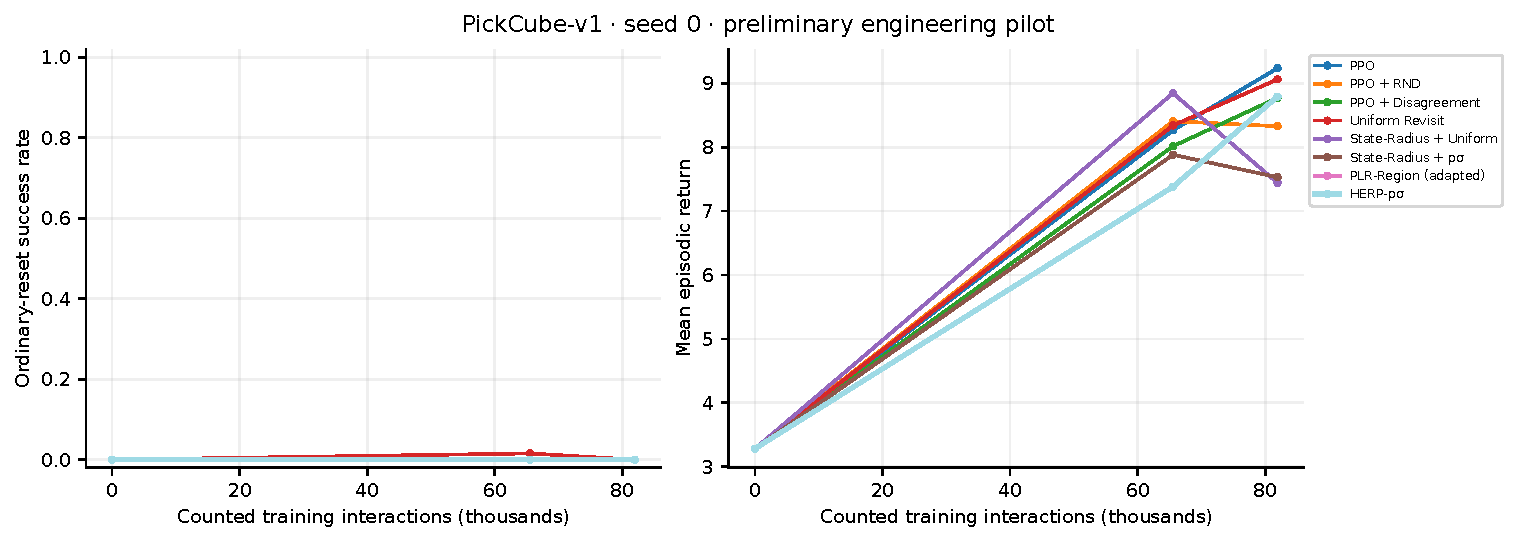
\includegraphics[width=\linewidth]{learning_curves.pdf}
\newpage
\section*{Method and acquisition diagnostics}
Behavioral boundaries use symmetric diagonal-Gaussian policy KL. Regions cluster normalized entry contexts, preserving the separation between acquisition source and current chain region. Fixed-window future dispersion estimates
\[
 \widehat q_v=\frac{1}{K_v(K_v-1)}\sum_{i<j}d_M(\xi_i,\xi_j),
 \qquad n_v\propto p_v\sqrt{\widetilde q_v+\epsilon_\sigma^2}.
\]
Complete, independent windows support the unbiased U-statistic interpretation. Every independent fragment has its own GAE boundary; artificial ends bootstrap and true terminations do not.

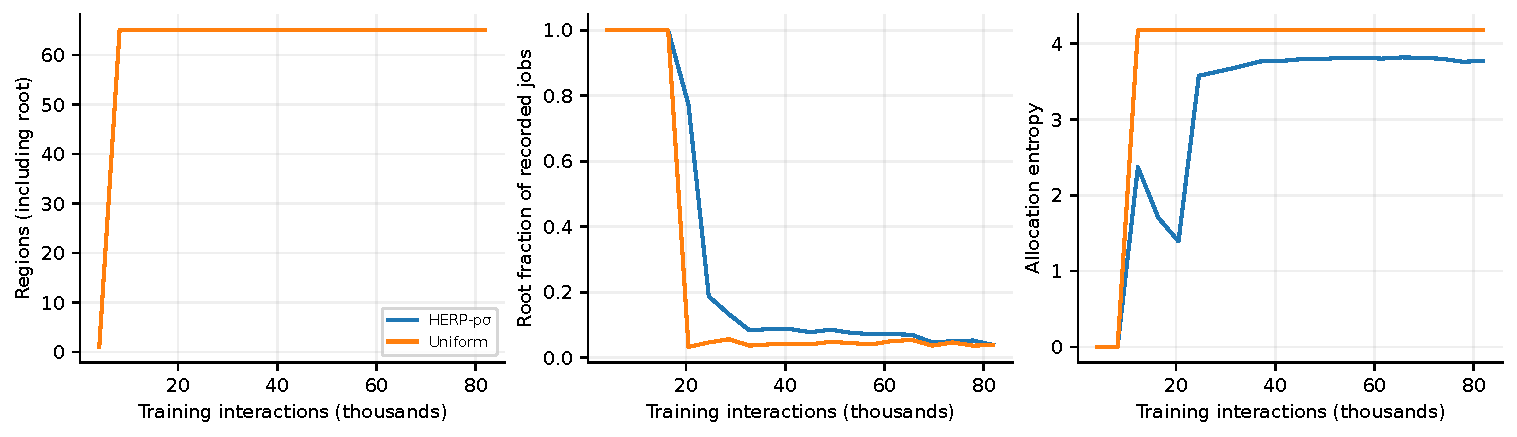
\includegraphics[width=\linewidth]{allocation_diagnostics.pdf}

\section*{Mechanism validation}
Independent-pool frozen-policy analysis is available for 25 successfully collected regions from the development HERP checkpoint. Collection stopped on a restore-consistency failure in a later region; the atomic saved pool is intact. These are exploratory pre-correction mechanism results. Direct and learned estimators use the same held-out regions. Resampling variability is not training-seed uncertainty. The controlled PPO-delta relevance gate has not yet been established.

\IfFileExists{sigma_mechanism.pdf}{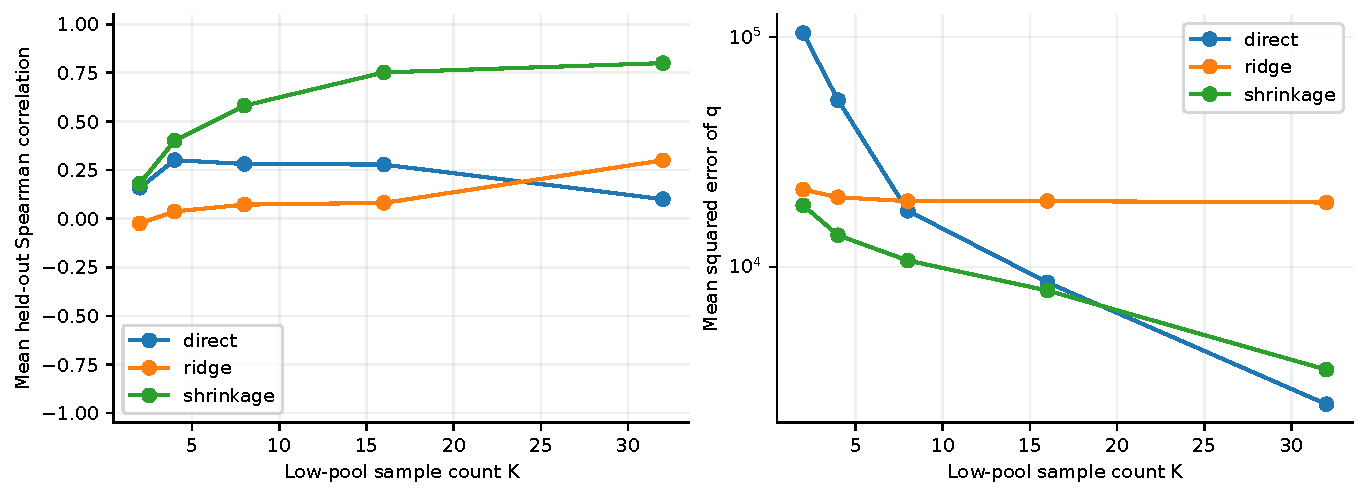
\includegraphics[width=\linewidth]{sigma_mechanism.pdf}}{}

\section*{Reproducibility and limits}
The runtime is Miniconda \texttt{deeplearning}, PyTorch 2.11.0+cu128, ManiSkill 3.0.1 and SAPIEN 3.0.3 on a GTX 1650 with 4 GB VRAM. WSL requires \texttt{LD\_LIBRARY\_PATH=/usr/lib/wsl/lib}. Raw simulator throughput at 512 environments was approximately 4,717 transitions/s; training wall time also includes collection processing and optimization.

Snapshots include controller state, clocks and contact-derived observation history. The non-contact CPU replay test measured next-observation error $5.36\times10^{-7}$. This does not prove exact serialization of contact-solver internals. Early development runs that failed restoration checks are excluded.

Root child-entry total variance is a proxy, not automatically an exact root-time conditional decomposition. Missing child means use a logged prior. PLR-Region and SACL-style are labelled adaptations; the latter uses fixed-state value change without a critic-uncertainty term.

One seed and one task cannot establish statistical superiority or cross-task generalization. Official RFCL, Active RL, BRO and MaxInfoRL repositories were downloaded and commit-locked, but their baseline results are not available. The remaining priority is mechanism acceptance, longer equal-budget runs, task coverage, then additional seeds.
\end{document}
